\section{Conclusions}

\begin{frame}{Conclusions and Future Works}
	\begin{itemize}
		\item For now \ldots
		\begin{itemize}
			\item The agent learns sub-optimal trajectory 
			\item A not-expert user can build IRL system
			\item Reward model emulates the human behavior
		\end{itemize}
	\end{itemize}
	
	\begin{columns}
		
		\begin{column}{0.33\textwidth}
			\includemedia[width=0.6\linewidth, passcontext, activate=pageopen, transparent, addresource=videos/IRLmvs.mp4, noplaybutton,
			deactivate=onclick,
			flashvars={source=videos/IRLmvs.mp4&autoPlay=true&loop=true}
			]{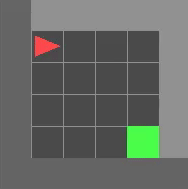
\includegraphics[width=0.6\linewidth]{videos/IRLmvs-1.png}}{VPlayer.swf}
		\end{column}
		
		\begin{column}{0.33\textwidth}
			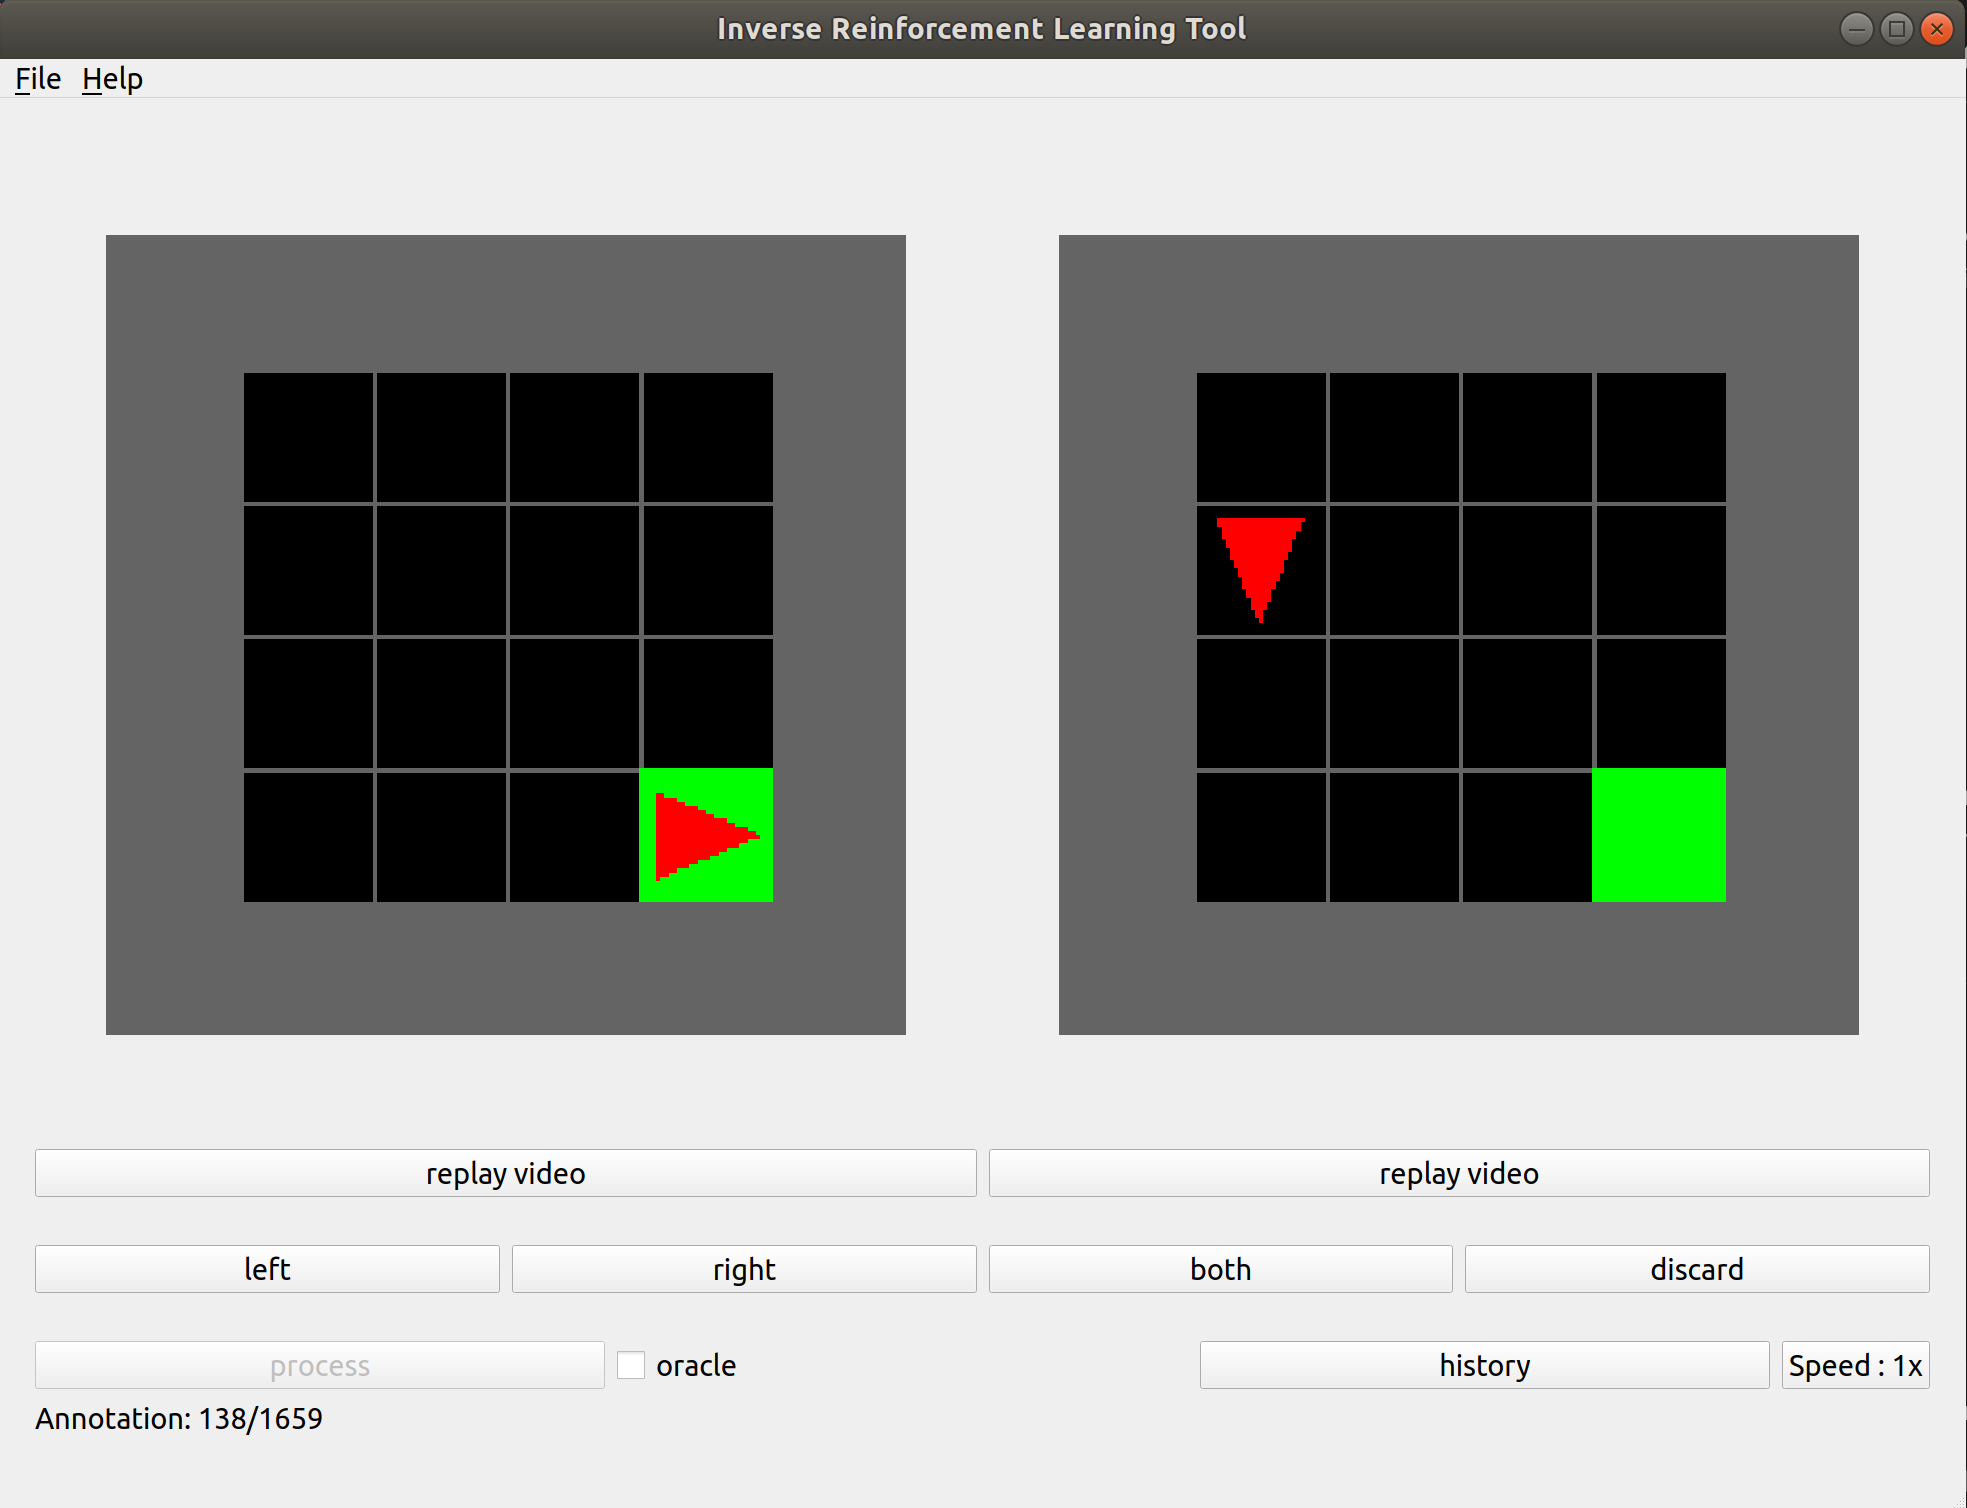
\includegraphics[width=0.8\linewidth]{images/alg_view.png}
		\end{column}
	
	
		\begin{column}{0.33\textwidth}
			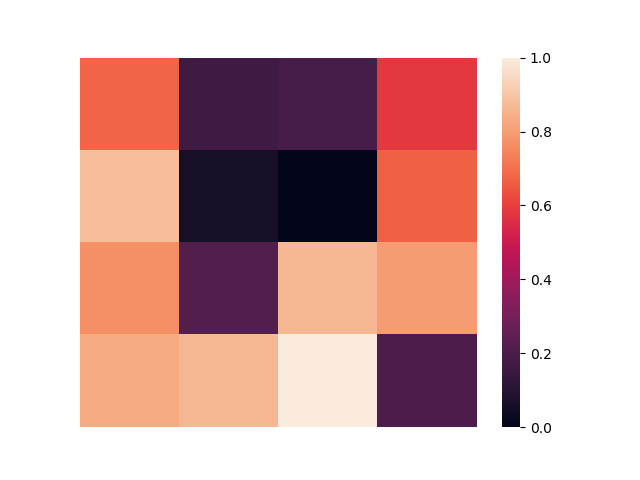
\includegraphics[width=\linewidth]{images/max_heatmap.png}
		\end{column}
	\end{columns}
	
	
	\begin{itemize}
		\item \ldots then
		\begin{itemize}
			\item More complex environment to increase IRL benefits
			\item Process environment images with agent states (with CNN and/or LSTM)
		\end{itemize}
	\end{itemize}
	
\end{frame}


\begin{comment}
	
	\begin{frame}{Conclusions and Future Works}
	
	\begin{columns}
	
	\begin{column}{0.6\textwidth}
	
	\begin{itemize}
	\item For now \ldots
	\begin{itemize}
	\item A not-expert user can build IRL system
	\item The agent learns sub-optimal trajectory 
	\item Reward model emulates the human behavior
	\end{itemize}
	\end{itemize}
	
	\end{column}
	
	\begin{column}{0.4\textwidth}
	\centering
	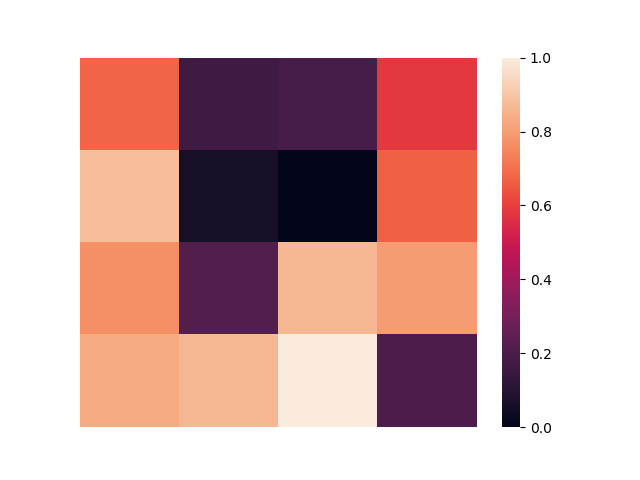
\includegraphics[width=0.7\linewidth]{images/max_heatmap.png}
	\end{column}
	
	\end{columns}
	
	
	
	\begin{itemize}
	\item<2-> \ldots then
	\begin{itemize}
	\item<2-> More complex environment to increase IRL benefits
	\item<2-> Process environment images with agent states (with CNN and/or LSTM)
	\end{itemize}
	\end{itemize}
	
	
	
	\end{frame}
\end{comment}
